\documentclass[a4paper, 12pt]{article}
\usepackage[T2A,T1]{fontenc}
\usepackage[utf8]{inputenc}
\usepackage[english, russian]{babel}
\usepackage{graphicx}
\graphicspath{{img/}}
\usepackage[hcentering, bindingoffset = 10mm, right = 15 mm, left = 15 mm, top=20mm, bottom = 20 mm]{geometry}
\usepackage{amsmath, amstext}
\usepackage{float}
\usepackage{wasysym}
\setlength{\parindent}{0em}
\setlength{\parskip}{0.5em}
\renewcommand{\arraystretch}{1.2}

\newenvironment{bottompar}{\par\vspace*{\fill}}{\clearpage}
 
\begin{document}

\begin{titlepage}
\newcommand{\HRule}{\rule{\linewidth}{0.5mm}} % Defines a new command for the horizontal lines, change thickness here

\center % Center everything on the page
 
\textsc{\LARGE Московский\\[-0.2cm]Физико-Технический Институт\\[0.1cm]\large (государственный университет)}\\[1.5cm] % Name of your university/college
\textsc{\Large Кафедра общей физики}\\[0.1cm] % Major heading such as course name
\textsc{\large Вопрос по выбору, 3 семестр}\\[0.5cm] % Minor heading such as course title

\HRule
\\[0.8cm]
{ \huge \bfseries Измерение удельного\\[0.3cm] сопротивления воздуха}
\\[0.8cm] % Title of your document
\HRule
\\[1.5cm]

\begin{flushleft} \large
	\textsf{Студент}\\[0.1cm]
	Ушаков Роман \\
	513 группа
\end{flushleft}

\begin{bottompar}
	\begin{center}
		
\includegraphics[width = 80 mm]{logo.jpg}
	\end{center}
	{\large \today}

\end{bottompar}
\vfill
\end{titlepage}

\subsection*{Цель работы}
Измерение удельного сопротивления воздуха.

\subsection*{Оборудование}
Линейка, карандаш, нить, два шарика для настольного тенниса, секундомер, резиновый или пластиковый предмет, который удобно электризовать (воздушный шарик <<ФАКИ>>).


\subsection*{Теория}
Заряд уединенного заряженного шарика, подвешенного на тонкой нити в воздухе, с течением времени уменьшается. Это связано с конечной величиной удельного сопротивления воздуха $\rho$. Запишем закон Ома в дифференциальной форме:
\begin{equation}
\vec{j} = \vec{E}/\rho.
\end{equation}

Теперь найдём величину тока разрядки:
\begin{equation}
I = \oiint_S \vec{j} \,\vec{dS} = \frac{1}{\rho}\oiint_S \vec{E} \,\vec{dS} = \dfrac{4 \pi q}{\rho}.
\end{equation}

Во втором переходе применена теорема Гаусса: $\oiint_S \vec{E} \,\vec{dS} = 4 \pi q$. Учитывая, что $I = -\dot q$, получаем дифференциальное уравнение:
\begin{equation}
\frac{dq}{dt} = - \frac{q}{\rho \varepsilon_0},
\end{equation}
решением которого является функция $q(t) = q_0  e^{-t/\tau}$, где $q_0$~---
начальный заряд шарика, $\tau = \varepsilon_0 \rho$~---~время, за которое заряд мячика уменьшается в $e$ раз. 

Тогда $\rho$ выражается через время \emph{полуразрядки} $T_{1/2}$:
\begin{equation}
\rho = \frac{T_{1/2}}{\varepsilon_0 \ln 2}.
\end{equation}

Заметим, что закон Кулона неприменим в данных условиях вследствие неравномерности распределения индуцированных зарядов на шариках.

\begin{figure}[H]
\begin{center}
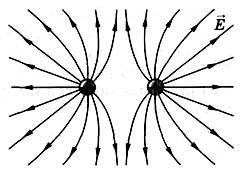
\includegraphics[width=0.6\textwidth]{7}
\end{center}
\end{figure}

\subsection*{Эксперимент}
Покроем теннисные шарики слоем графита (используя карандаш и упорство), затем подвесим их так, чтобы расстояние между нитями равнялось диаметру шарика $d_0=2R=40$~мм. Длина нитей $L=140$~cм. Незаряженные шарики должны слегка соприкасаться. С помощью линейки будем измерять расстояние между шариками.

\begin{figure}[h]\centering
\begin{center}
\begin{minipage}[h]{0.45 \linewidth}
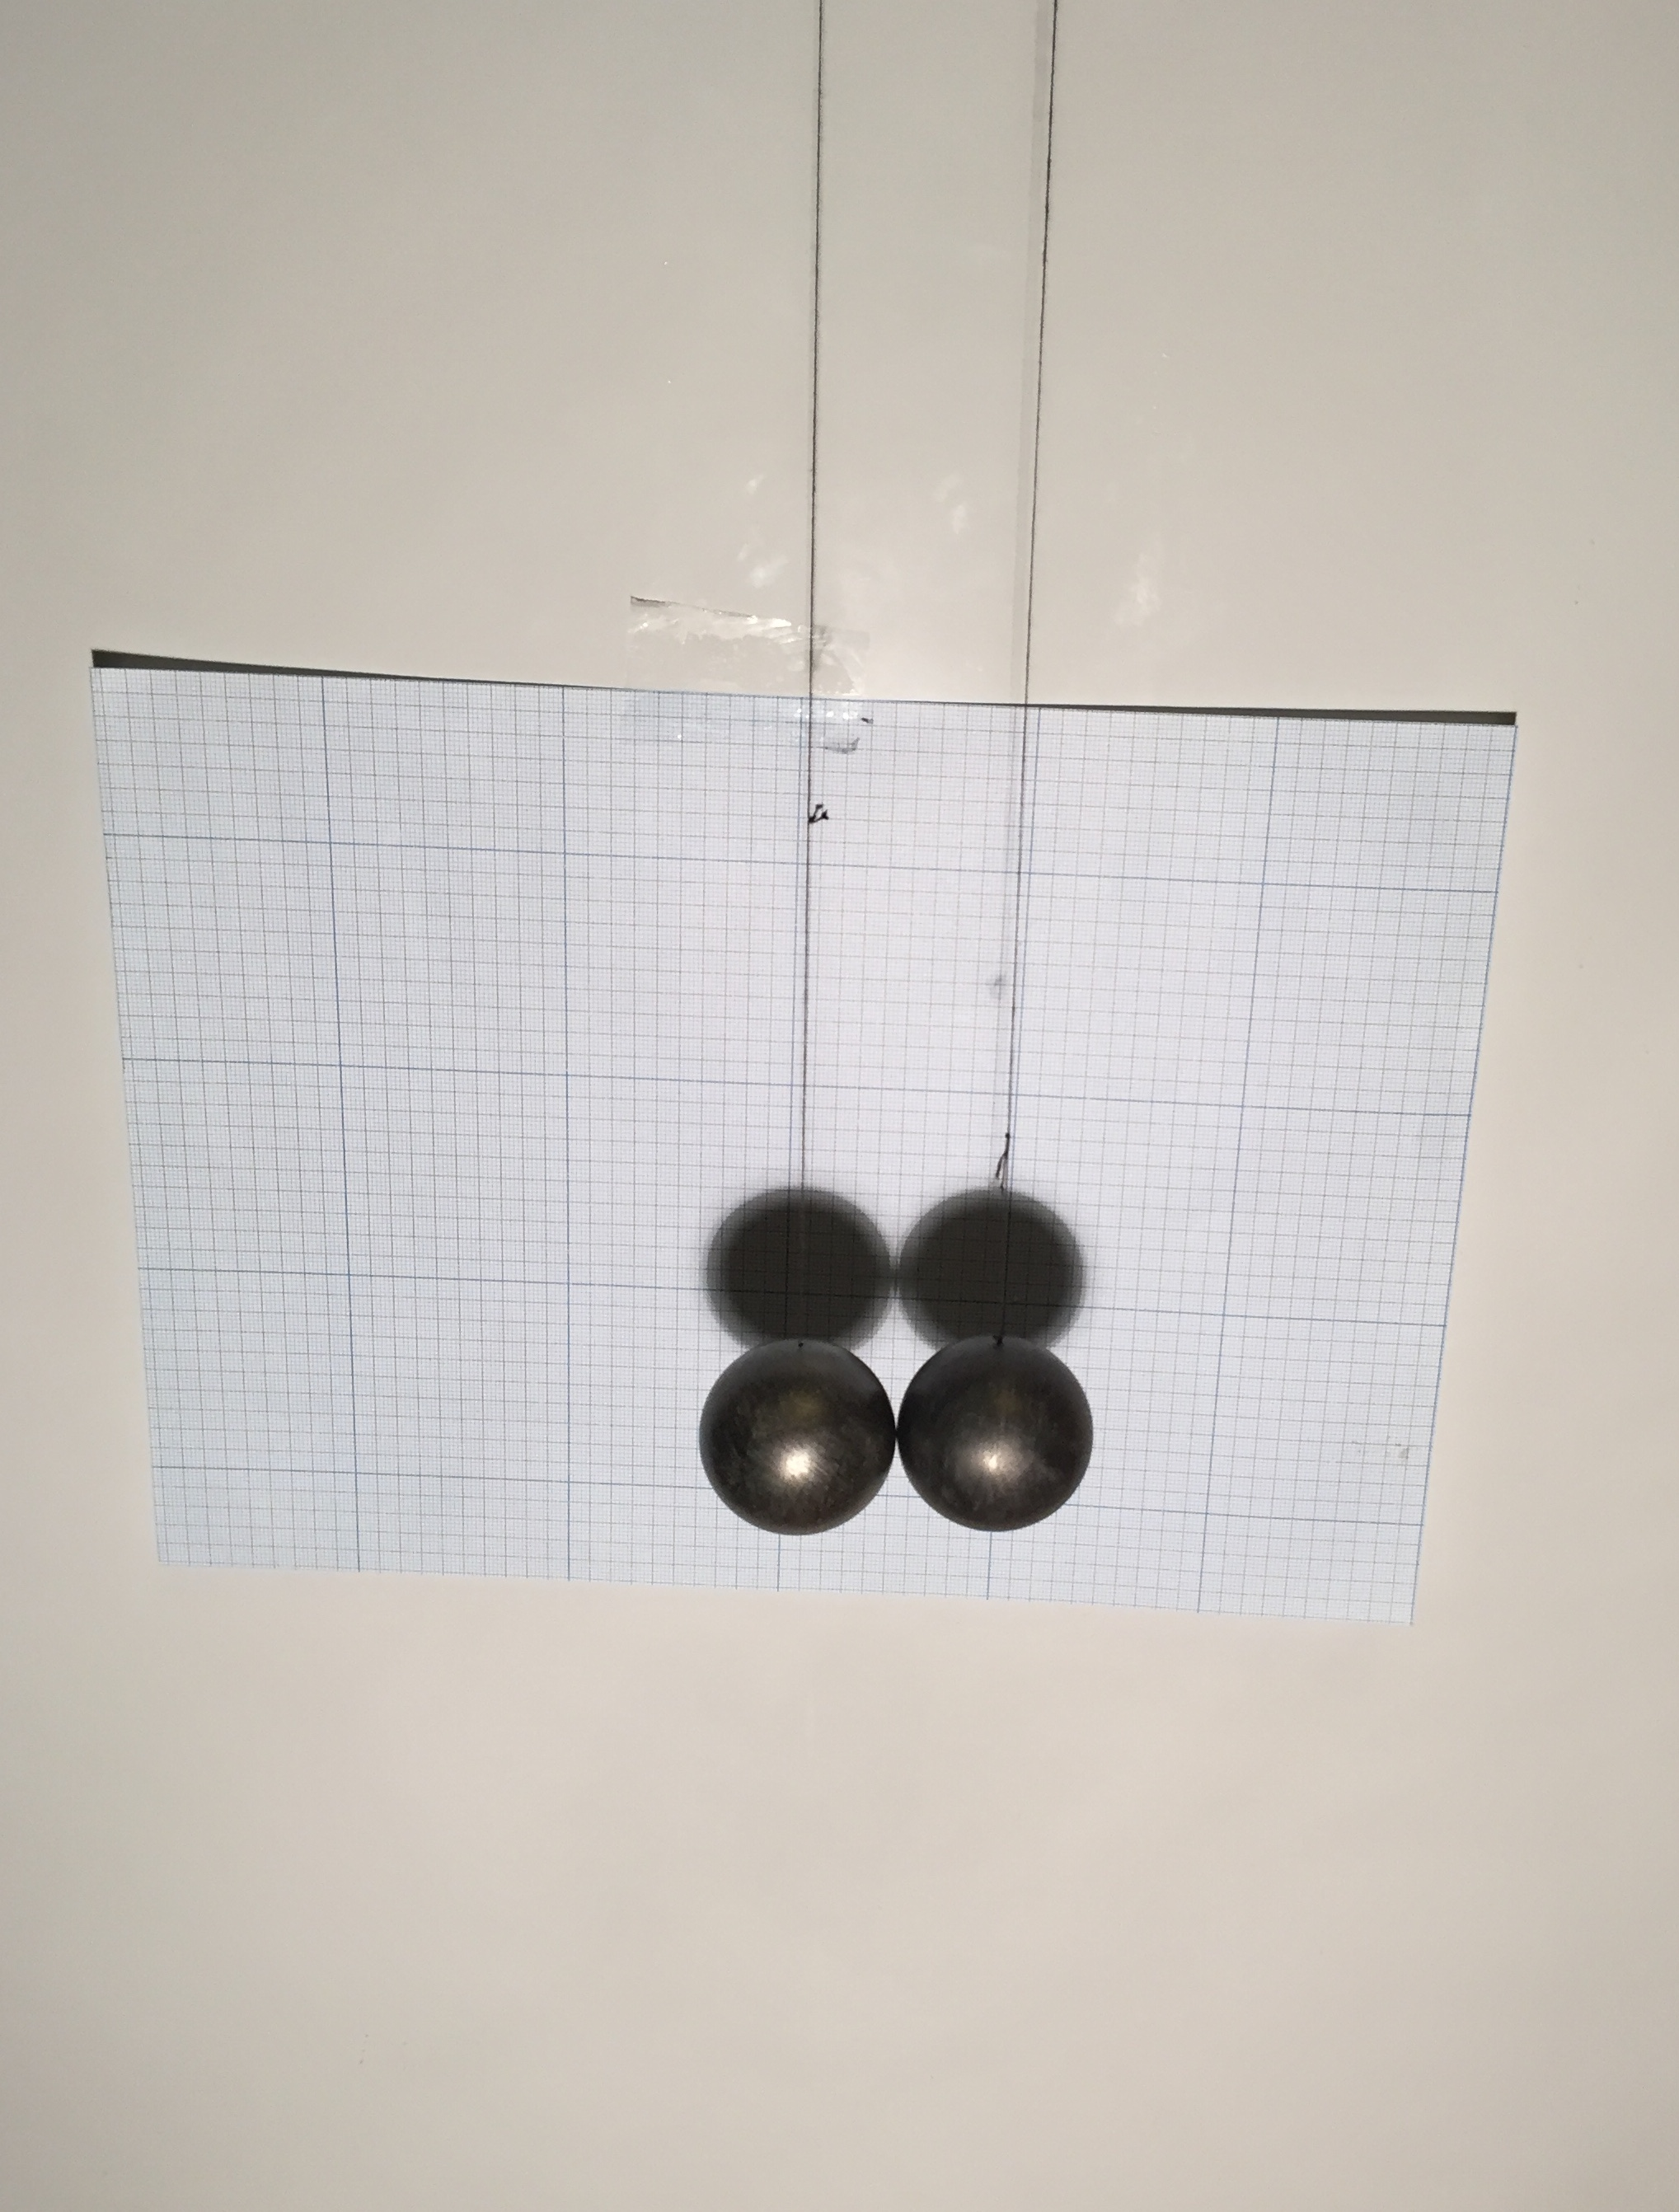
\includegraphics[height=10cm]{3}
\end{minipage}
\qquad
\begin{minipage}[h]{0.45 \linewidth}
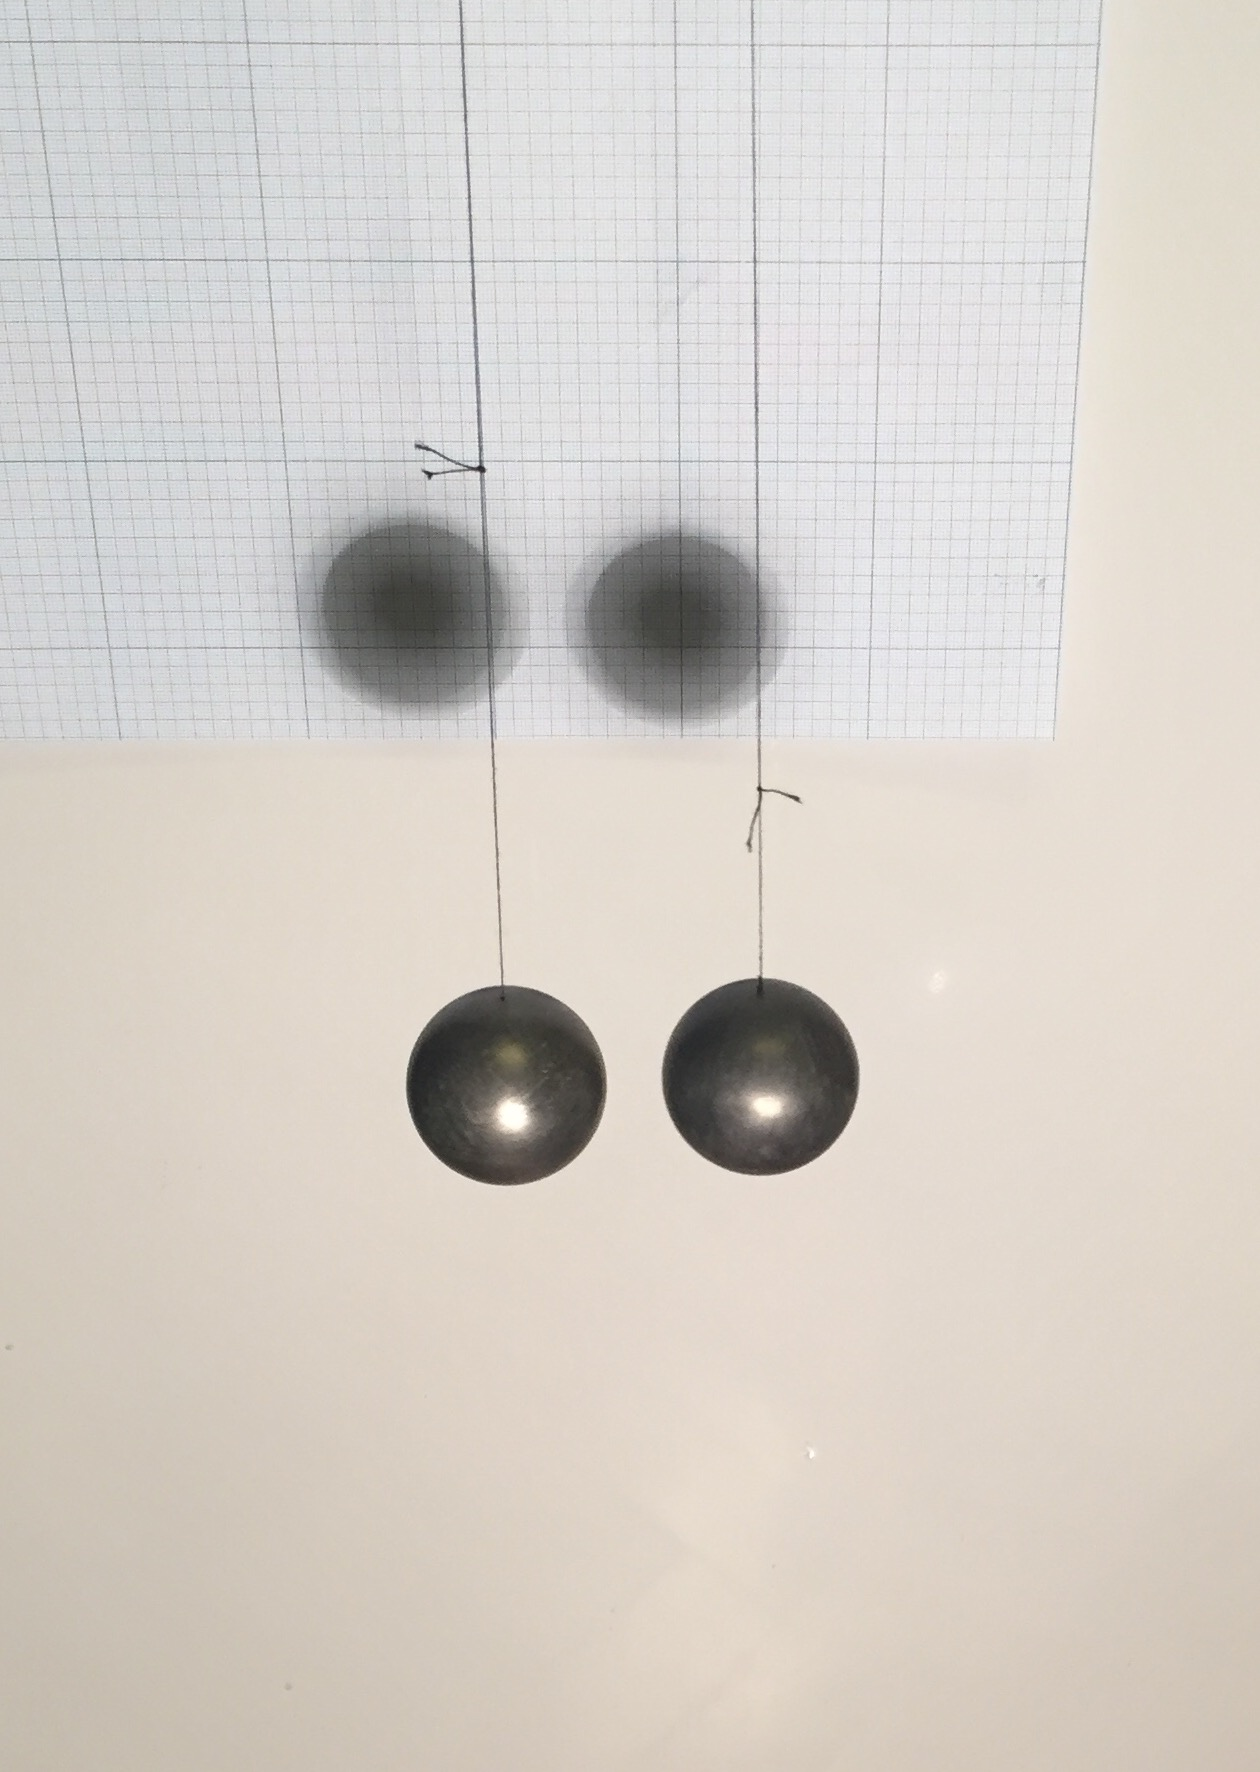
\includegraphics[height=10cm]{5}
\end{minipage}
\end{center}
\end{figure}
\vspace{-.4cm}

\subsection*{Калибровка установки}
Заряжаем теннисные мячики с помощью воздушного шарика «ФАКИ» и измеряем расстояние между нитями на высоте $10$~см от шариков $d_1$. Затем разряжаем один из шариков, касаясь его рукой. После соударения шарики снова расходятся (их заряды при этом вдвое меньше, чем изначально), но на этот раз расстояние составляет $d_2$. Калибровка проведена.

Вновь заряжаем шарики так, что расстояние между нитями, отсчитанное по линейке, было равным $d_1$, и с помощью секундомера измеряем время $T_{1/2}$, за которое расстояние между нитями уменьшается до $d_2$.


\subsection*{Измерения}

I серия опытов:~ $d_1 = 73$ мм ~$\longrightarrow$~ $d_2 = 41$ мм.

\begin{tabular}{|l|r|r|r|r|r|r|r|r|r|}
\hline
№ & 1 & 2 & 3 & 4 & 5 & 6 & 7 & 8 & 9 \\
\hline
$T_{1/2}$, с & 468 & 471 & 474 & 490 & 463 & 453 & 448 & 501 & 451 \\
\hline
$\rho$, $10^{13}$ Ом $\cdot$ м & 7.6 & 7.6 & 7.7 & 8.0 & 7.5 & 7.4 & 7.3 & 8.2 & 7.4\\
\hline
\end{tabular}

\clearpage

II серия опытов:~ $d_1 = 78$ мм ~$\longrightarrow$~ $d_2 = 43$ мм.

\begin{tabular}{|l|r|r|r|r|r|r|r|r|r|r|}
\hline
№ & 1 & 2 & 3 & 4 & 5 & 6 & 7 & 8 & 9 \\
\hline
$T_{1/2}$, с & 498 & 546  & 489 & 462 & 473 & 476 & 489 & 457 & 486  \\
\hline
$\rho$, $10^{13}$ Ом $\cdot$ м & 8.1 & 8.9 & 8.0 & 7.5 & 7.7 & 7.8 & 8.0 & 7.5 & 8.0\\
\hline
\end{tabular}

\bigskip

III серия опытов:~ $d_1 = 76$ мм ~$\longrightarrow$~ $d_2 = 42$ мм.

\begin{tabular}{|l|r|r|r|r|r|r|r|r|r|r|}
\hline
№ & 1 & 2 & 3 & 4 & 5 & 6 & 7 \\
\hline
$T_{1/2}$, с & 475  & 467 & 474 & 497  & 435 & 449 & 478  \\
\hline
$\rho$, $10^{13}$ Ом $\cdot$ м & 7.8 & 7.6 & 7.7 & 8.1 & 7.0  & 7.3 & 7.8\\
\hline
\end{tabular}

\bigskip

В результате имеем
\begin{eqnarray}
\rho &=& 7.7 \cdot 10^{13}~\text{Ом} \cdot \text{м},\\
\sigma_{T_{1/2}} = 23~\text{c} ~~~\Rightarrow~~~ \sigma_{\rho} &=& 0.4\cdot 10^{13}~\text{Ом} \cdot \text{м}.
\end{eqnarray}

Следует отметить, что реальная величина удельного сопротивления воздуха существенно зависит от температуры и влажности и колеблется в диапазоне $\rho = 10^{13} \div 10^{15}$ Ом $\cdot$ м. 

\subsection*{Вывод}
В данной работе был продемонстрирован способ измерения удельного сопротивления воздуха. Однако данный способ применим не только к воздуху, но и к любым слабо ограниченным средам, в которых выполняется закон Ома.

Важно заметить, что при анализе результатов эксперимента не используется закон Кулона, поскольку заряженные шарики нельзя считать точечными зарядами: поверхностные заряды на них имеют сложную конфигурацию. 

\subsection*{Источники}

[1] \textit{Д.\,В. Сивухин.} Общий курс физики. Электричество

\vspace{-.7\parskip}
[2] \textit{А.\,В. Гуденко.} Удельное сопротивление воздуха /\!/ T2--11A. IEPhO, 2015


\end{document}